%\documentclass{article}
%
%\usepackage{fancyhdr}
%\usepackage{extramarks}
%\usepackage{amsmath}
%\usepackage{amsthm}
%\usepackage{amsfonts}
%\usepackage{tikz}
%\usepackage{enumerate}
%\usepackage{graphicx}
%\graphicspath{ {images/} }
%\usepackage[plain]{algorithm}
%\usepackage{algpseudocode}
%\usepackage[document]{ragged2e}
%\usepackage{textcomp}
%\usepackage{color}   %May be necessary if you want to color links
%\usepackage{import}
%\usepackage{hyperref}
%\hypersetup{
%    colorlinks=true, %set true if you want colored links
%    linktoc=all,     %set to all if you want both sections and subsections linked
%    linkcolor=black,  %choose some color if you want links to stand out
%}
%
%\usetikzlibrary{automata,positioning}
%
%%
%% Basic Document Settings
%%
%
%\topmargin=-0.45in
%\evensidemargin=0in
%\oddsidemargin=0in
%\textwidth=6.5in
%\textheight=9.0in
%\headsep=0.25in
%\setlength{\parskip}{1em}
%
%\linespread{1.1}
%
%\pagestyle{fancy}
%\lhead{\hmwkAuthorName}
%\lfoot{\lastxmark}
%\cfoot{\thepage}
%
%\renewcommand\headrulewidth{0.4pt}
%\renewcommand\footrulewidth{0.4pt}
%
%\setlength\parindent{0pt}
%
%
%\newcommand{\hmwkTitle}{Math Review Notes---Linear Algebra}
%\newcommand{\hmwkAuthorName}{\textbf{G. Faletto} }
%
%%
%% Title Page
%%
%
%\title{
%    \vspace{2in}
%    \textmd{\textbf{ \hmwkTitle}}\\
%}
%
%\author{Gregory Faletto}
%\date{}
%
%\renewcommand{\part}[1]{\textbf{\large Part \Alph{partCounter}}\stepcounter{partCounter}\\}
%
%%
%% Various Helper Commands
%%
%
%% Useful for algorithms
%\newcommand{\alg}[1]{\textsc{\bfseries \footnotesize #1}}
%
%% For derivatives
%\newcommand{\deriv}[2]{\frac{\mathrm{d} #1}{\mathrm{d} #2}}
%
%% For partial derivatives
%\newcommand{\pderiv}[2]{\frac{\partial #1}{\partial #2}}
%
%% Integral dx
%\newcommand{\dx}{\mathrm{d}x}
%
%% Alias for the Solution section header
%\newcommand{\solution}{\textbf{\large Solution}}
%
%% Probability commands: Expectation, Variance, Covariance, Bias
%\newcommand{\E}{\mathbb{E}}
%\newcommand{\Var}{\mathrm{Var}}
%\newcommand{\Cov}{\mathrm{Cov}}
%\newcommand{\Bias}{\mathrm{Bias}}
%\newcommand\indep{\protect\mathpalette{\protect\independenT}{\perp}}
%\def\independenT#1#2{\mathrel{\rlap{$#1#2$}\mkern2mu{#1#2}}}
%\DeclareMathOperator{\Tr}{Tr}
%
%\theoremstyle{definition}
%\newtheorem{theorem}{Theorem}
%\numberwithin{theorem}{subsection}
%\theoremstyle{definition}
%\newtheorem{proposition}[theorem]{Proposition}
%\theoremstyle{definition}
%\newtheorem{lemma}[theorem]{Lemma}
%\theoremstyle{definition}
%\newtheorem{corollary}{Corollary}[theorem]
%\theoremstyle{definition}
%\newtheorem{definition}{Definition}[section]
%\newtheorem*{remark}{Remark}
%\theoremstyle{definition}
%\newtheorem{exercise}{Exercise}
%
%% Tilde
%\newcommand{\textapprox}{\raisebox{0.5ex}{\texttildelow}}
%
%\begin{document}
%
%\maketitle
%
%\pagebreak
%
%\tableofcontents
%
%\
%
%\
%
%\begin{center}
%Last updated \today
%\end{center}
%
%\newpage
%
%%
%%
%%
%%
%%
%%
%%

\chapter{Linear Algebra}\label{sec.lin.alg}

These are my notes from taking EE 588 at USC, Math 541A at USC, and various other sources which I mostly cite within the text. (For more notes on linear algebra, see Section \ref{ra.lin.alg.5.1.pugh}.)

\section{Properties of Projection Matrices}

\begin{enumerate}[i.]

\item Formula:

\[
P = A(A^TA)^{-1}A^T
\]

(Note that if \(A\) is an invertible (square) matrix, then \(P = A(A^TA)^{-1}A^T = AA^{-1}(A^T)^{-1}A^T = I\).)

\textbf{The projection matrix projects any vector \(b\) into the column space of \(A\).} In other words, \(p = Pb\) is the component of \(b\) in the column space, and the error \(e = b - Pb\) is the component in the orthogonal complement. (\(I - P\) is also a projection matrix. It projects \(b\) onto the orthogonal complement, and the projection is \(b - Pb = e\)).

(Note that if \(A\) is an invertible (square) matrix, then its column space is all of \(\mathbb{R}^n\), so \(b\) is already in the column space of \(A\).)

\item The projection matrix is \textbf{idempotent}: it equals its square--\(P^2 = P\).

\item The projection matrix is \textbf{symmetric}: it equals its transpose--\(P^T = P\).

\item Conversely, \textbf{any symmetric idempotent matrix represents a projection}. \(P\) is unique for a given subspace.

\item If \(A\) is an \(m \times n\) matrix with rank \(n\), then \(\text{rank} (P) = n\). The eigenvalues of \(P\) consist of \(n\) ones and \(m - n\) zeroes. \(P\) always contains \(n\) independent eigenvectors and is thus diagonalizable. 

\end{enumerate}

Suppose \(A\) is a square nonsingular matrix and \(\lambda\) is an eigenvalue of \(A\). Then \(\lambda^{-1}\) is an eigenvalue of the matrix \(A^{-1}\).

\begin{proposition}

The eigenvalues of an idempotent matrix equal either 0 or 1.

\end{proposition}

\begin{proof}

Let \(A\) be an idempotent matrix and let \(v\) be a unit-length eigenvector of \(H\) with corresponding eigenvalue \(\lambda\). Then

\[
Av = \lambda v \implies A (Av) = A (\lambda v) .
\]

Then

\[
AAv = Av = \lambda v
\]

and

\[
\lambda A v = \lambda^2 v
\]

so we have

\[
\lambda v = \lambda^2 v \implies \lambda \in \{0, 1\}.
\]

\end{proof}

The trace of an idempotent matrix with rank \(r\) is \(r\).

\begin{theorem}[\textbf{Math 425b Homework Problem}]

Let \((V, \langle \cdot, \cdot \rangle)\) be a real or complex vector space. Let \(W\) be a finite-dimensional subspace of \(V\) with an orthonormal basis \(\{w_1, \ldots, w_n\}\). For \(v \in V\), define the orthogonal projection of \(v\) onto \(W\) to be

\[
\operatorname{proj}_W(v) :=  \sum_{i=1}^n \langle w_i, v \rangle w_i.
\]

Then \(\operatorname{proj}_W(v)  \in W\) and \(v - \operatorname{proj}_W(v) \in W^\perp\), where \(W^\perp\) is the orthogonal complement of \(W\). Further, these properties characterize \(\operatorname{proj}_W(v) \) of uniquely; i.e., if \(v = v_1 + v_2 = v-1' + v_2'\) with \(v_1, v_1' \in W\) and \(v_2, v_2' \in W^\perp\) then \(v_1 = v_1'\) and \(v_2 = v_2'\).

\end{theorem}

\begin{proof}

Since \(\{w_1, \ldots, w_n\}\) is a basis for for \(W\), it holds that \(\operatorname{proj}_W(v) \in W\) if and only if for some \((c_1, \ldots, c_n) \in \mathbb{R}^n\) it holds that \( \operatorname{proj}_W(v) = \sum_{i=1}^n c_i w_i\). But

\[
 \operatorname{proj}_W(v) =  \sum_{i=1}^n \langle w_i, v \rangle w_i
\]

so this follows from \(c_i := \langle w_i, v \rangle, i \in [n]\). Next we will show that \(v - \operatorname{proj}_W(v) \in W^\perp\). This is true if and only if \(\langle w, v - \operatorname{proj}_W(v) \rangle = 0\) for all \(w \in W\). Let \(w \in W\) be expressed as \(\sum_{j=1}^n c_j w_j\) for some \((c_1, \ldots, c_n) \in \mathbb{R}^n\). Note that since \(\{w_1, \ldots, w_n\}\) is an orthonormal basis, \(\langle w_j, w_i \rangle = \delta_{j,i}\). Then

\begin{align*}
\langle w, v - \operatorname{proj}_W(v) \rangle &  = \langle w, v  \rangle - \langle w, \operatorname{proj}_W(v) \rangle 
\\ & = \left\langle \sum_{j=1}^n c_j w_j,  v \right\rangle - \left\langle \sum_{j=1}^n c_j w_j, \sum_{i=1}^n \langle w_i, v \rangle w_i. \right\rangle
\\ & = \sum_{j=1}^n  c_j \left\langle  w_j,  v \right\rangle -\sum_{j=1}^n c_j  \left\langle  w_j, \sum_{i=1}^n \langle w_i, v \rangle w_i. \right\rangle
\\ & = \sum_{j=1}^n  c_j \left\langle  w_j,  v \right\rangle -\sum_{j=1}^n \sum_{i=1}^n c_j  \langle w_i, v \rangle \left\langle  w_j,  w_i. \right\rangle
\\ & = \sum_{j=1}^n  c_j \left\langle  w_j,  v \right\rangle -\sum_{j=1}^n \sum_{i=1}^n c_j  \langle w_i, v \rangle \delta_{j,i}
\\ & = \sum_{j=1}^n  c_j \left\langle  w_j,  v \right\rangle - \sum_{j=1}^n c_j  \langle w_j, v \rangle 
\\ & = 0,
\end{align*}

where we used elementary properties of inner products. Lastly, we will show that these properties characterize \( \operatorname{proj}_W(v)\) uniquely. Let \(v_1, v_1' \in W\) and \(v_2, v_2' \in W^\perp\). In particular, let \(v_1 = \sum_{i=1}^n c_i w_i\) and \(v_1' = \sum_{i=1}^n c_i' w_i\), and note that \(\langle w_j , v_2 \rangle = \langle w_j, v_2' \rangle = 0\) for all \(j \in [n]\). Suppose \(v_1 + v_2 = v_1' + v_2'\). Then for all \(j \in [n]\),

\begin{align}
& 0 = v_1 + v_2 - (v_1' + v_2') =  \sum_{i=1}^n \left(  c_i  - c_i'   \right)  w_i + v_2 - v_2' \label{linalg.425b.hw7.e}
\\ \implies \qquad & \langle w_j, 0 \rangle = \left\langle w_j, \sum_{i=1}^n \left(  c_i  - c_i'   \right)  w_i + v_2 - v_2'  \right \rangle 
%\\ \qquad & 
=  \sum_{i=1}^n \left\langle w_j, \left(  c_i  - c_i'   \right)  w_i  \right \rangle +\left\langle w_j, v_2  \right \rangle -  \left\langle w_j, \ v_2'  \right \rangle \nonumber
\\ \implies \qquad & 0 = c_j - c_j', \nonumber
\end{align} 

so \(v_1 = v_1'\). Then from (\ref{linalg.425b.hw7.e}) we have

%Further, since by the above \(\langle w_j, v - \operatorname{proj}_W(v)
%\rangle = 0\) for any \(v \in V\) and all \(j \in [n]\), we have from (\ref{linalg.425b.hw7.e})

\[
0 = v_2 - v_2' \qquad \iff v_2 = v_2'.
\]


%\begin{align*}
%&  0 - \operatorname{proj}_W(0) =  \sum_{i=1}^n \left(  c_i  - c_i'   \right)  w_i + v_2 - v_2' - \operatorname{proj}_W \left( \sum_{i=1}^n \left(  c_i  - c_i'   \right)  w_i + v_2 - v_2' \right)
%\\ \implies \qquad & =
%\end{align*} 



\end{proof}

\begin{theorem}[\textbf{Math 425b Homework Problem}]

Let \((V, \langle \cdot, \cdot \rangle)\) be a real or complex vector space. Let \(W\) be a finite-dimensional subspace of \(V\) with an orthonormal basis \(\{w_1, \ldots, w_n\}\). For \(v \in V\), define the orthogonal projection of \(v\) onto \(W\) to be

\[
\operatorname{proj}_W(v) :=  \sum_{i=1}^n \langle w_i, v \rangle w_i.
\] 

Then \( \operatorname{proj}_W(v)\) is the closest element of \(W\) to \(v\) (in \(L_2\) norm). That is, for any \(w \in W\) we have \(\lVert v -  \operatorname{proj}_W(v) \rVert_2 \leq  \lVert v - w \rVert_2 \).

\end{theorem}

\begin{proof}

For any \(w \in W\),

%\[
%v - w = 
%\]
%
\begin{align*}
& v - w = v - \operatorname{proj}_W(v) + \operatorname{proj}_W(v) - w 
\\ \implies \qquad & \lVert v - w \rVert_2^2 =  \lVert v - \operatorname{proj}_W(v)  \rVert_2^2 +  \lVert \operatorname{proj}_W(v) - w  \rVert_2^2 + 2 \lVert ( v - \operatorname{proj}_W(v)) ( \operatorname{proj}_W(v) - w ) \rVert_2^2
\\ \implies \qquad & \lVert v - w \rVert_2^2 \geq  \lVert v - \operatorname{proj}_W(v)  \rVert_2^2 
\\ \iff \qquad & \lVert v - w \rVert_2 \geq  \lVert v - \operatorname{proj}_W(v)  \rVert_2.
\end{align*}
%
%\[
% \lVert v - w \rVert_2^2 =  \lVert v - \operatorname{proj}_W(v)  \rVert_2^2 +  \lVert \operatorname{proj}_W(v) - w  \rVert_2^2 + 2 \lVert ( v - \operatorname{proj}_W(v)) ( \operatorname{proj}_W(v) - w ) \rVert_2^2
% \]

\end{proof}

\section{Eigenvalues, Eigenvectors, Diagonalization, Symmetric Matrices}

\textbf{Notes on Diagonalization}

Suppose the \(n \times n\) matrix \(A\) has \(n\) linearly independent eigenvectors. If these eigenvectors are the columns of a matrix \(S\), then \(S^{-1}AS\) is a diagonal matrix \(\Lambda\). The eigenvalues of \(A\) are on the diagonal of \(\Lambda\):

\[
S^{-1}AS = \Lambda = \begin{bmatrix}
   \lambda_1       & 0  & \cdots  & 0  \\
  0  & \lambda_2 & \cdots  & 0 \\
  \vdots  & \vdots  & \ddots & \vdots \\
   0  & 0 & \cdots & \lambda_n
\end{bmatrix}
\]

We call \(S\) the \textbf{eigenvector matrix} and \(\Lambda\) the \textbf{eigenvalue matrix}.

\begin{enumerate}[1.]

\item If the matrix \(A\) has no repeated eigenvalues, then its \(n\) eigenvectors are automatically independent. Therefore \textbf{any matrix with \(n\) distinct eigenvalues can be diagonalized}.

\item \textbf{The diagonalizing matrix \(S\) is not unique}. An eigenvector \(x\) can be multiplied by a constant and remains an eigenvector. We can multiply the columns of \(S\) by any nonzero constants and produce a new diagonalizing \(S\). Repeated eigenvalues leave even more freedom in \(S\) (columns with identical eigenvalues can be interchanged). 

(Note that for the trivial example \(A = I\), any invertible \(S\) will do. \(S^{-1}IS\) is always diagonal, and \(\Lambda\) is just \(I\). \textbf{All vectors are eigenvectors of the identity.})

\item \textbf{Other matrices \(S\) will not produce a diagonal \(\Lambda\)}. Since \(\Lambda = S^{-1}AS\), \(S\) must satisfy \(S \Lambda = AS\). Suppose the first column of \(S\) is \(y\). Then the first column of \(S \Lambda\) is \(\lambda_1y\). If this is to agree with the first column of \(AS\), which by matrix multiplication is \(Ay\), then \(y\) must be an eigenvector: \(Ay = \lambda_1y\). 

(Note that the \textit{order} of the eigenvectors in \(S\) and the eigenvalues in \(\Lambda\) must match.)

\item Not all matrices posses \(n\) linearly independent eigenvectors, so \textbf{not all matrices are diagonalizable}. 

\textbf{Diagonalizability of \(A\) depends on having enough (\(n\)) independent eigenvectors. Invertibility of \(A\) depends on having nonzero eigenvalues.}

There is no connection between diagonalizability (\(n\) independent eigenvectors) and invertibility (no zero eigenvalues). The only indication given by the eigenvalues is that diagonalization can fail only if there are repeated eigenvalues. (But even then, it does not always fail--e.g. \(I\).)

The test is to check, for an eigenvalue that is repeated \(p\) times, whether there are \(p\) independent eigenvectors--in other words, whether \(A - \lambda\) has rank \(n - p\).

%If eigenvectors \(x_1, x_2, \ldots, x_k\) correspond to different eigenvalues \(\lambda_1, \lambda_2, \ldots, \lambda_k\), then those eigenvectors are linearly independent.

\item \textbf{Projection matrices always contain \(n\) independent eigenvectors and thus are always diagonalizable}.

\end{enumerate}

\textbf{Eigenvalues of Symmetric Matrices:} If \(A\) is symmetric, then it has the following properties:

\begin{enumerate}[1.]

\item \(A\) has exactly \(n\) (not necessarily distinct) eigenvalues

\item There exists a set of \(n\) eigenvectors, one for each eigenvalue, that are mutually orthogonal (even if the eigenvalues are not distinct).

\end{enumerate}

\textbf{Eigenvalues of the Inverse of a Matrix:} Suppose \(A\) is a square nonsingular matrix and \(\lambda\) is an eigenvalue of \(A\). Then \(\lambda^{-1}\) is an eigenvalue of the matrix \(A^{-1}\). Proof: Note that since \(A\) is nonsingular, \(A^{-1}\) exists and \(\lambda\) is nonnegative for all eigenvalues of \(A\). Let \(\lambda\) be an eigenvalue of \(A\) and let \(x \neq 0\) be an eigenvector of \(A\) for \(\lambda\). Suppose \(A\) is \(n\) by \(n\). Then we have

\[
A^{-1}x = A^{-1}\lambda^{-1} \lambda x = \lambda^{-1} A^{-1} \lambda x = \lambda^{-1} A^{-1} A x = \lambda^{-1}x
\]

\textbf{The inverse of a symmetric matrix is symmetric.} Proof: Let \(A\) be a symmetric matrix.

\[
I = I'
\]

\[
A A^{-1} = (A A^{-1})'
\]

\[
A^{-1} A = (A^{-1})'A'
\]

\[
A^{-1} A A^{-1} = (A^{-1})'A A^{-1}
\]

\[
A^{-1} = (A^{-1})'
\]

\section{Positive Definite Matrices}

\begin{proposition}\label{linalg.prop.inner.prod.psd}
For any real matrix \(A \in \mathbb{R}^{m \times n}\) with \(m \geq n\), the product \(A^T A\) is a positive semidefinite matrix. 

\end{proposition}

\begin{proof}
Let \(z\) be a non-zero vector. \(A^TA\) is positive semidefinite if and only if \(z^T A'^TA z \geq 0 \forall z \in \{ \mathbb{R}^n \setminus \{0\}\}\). Note that \(z^T A^T A z = (Az)^T(Az) = \lVert Az \rVert_2^2 \geq 0.\)

\end{proof}

\begin{proposition}
For any real invertible matrix \(A \in \mathbb{R}^{n \times n}\), the product \(A' A\) is a positive definite matrix. 

\end{proposition}

\begin{proof} Let \(z\) be a non-zero vector. \(A'A\) is positive definite if and only if \(z' A' A z >0 \forall z \in \{\mathbb{R}^n \setminus \{0\}\}\). Note that \(z' A' A z = (Az)'(Az)\). Because \(A\) is invertible and \(z \neq 0\), \(Az \neq 0 \), so \((Az)'(Az) = \lVert Az \rVert_2^2 > 0\).
\end{proof}



\begin{proposition}[\textbf{Math 547 Homework Problem}]
Let $A$ be an $m\times n$ real matrix with $m\geq n$. Then $A$ has rank $n$ if and only if $A^{T}A$ is positive definite.
\end{proposition}

\begin{proof}


By Proposition \ref{linalg.prop.inner.prod.psd}, \(A^TA\) is positive semidefinite. Since \(A^TA\) is not invertible if one of its eigenvalues equals 0, \(A^TA\) is invertible (and therefore full rank) if and only if it is positive definite. But \(A^TA \in \mathbb{R}^{n \times n}\) is full rank if and only if the columns of \(A\) are linearly independent, for the following reason: multiplying \(A^TA\) means taking linear combinations of the rows of \(A^T\) (that is, the columns of \(A\)) one at a time, with weightings according to the columns of \(A\). These linear combinations will themselves be linearly independent if and only if the rows of \(A^T\) (the columns of \(A\)) are linearly independent and for the basis of an \(n\)-dimensional subspace. And \(A^TA\) has linearly independent columns if and only if it is invertible.

So we have shown that \(A^TA\) is positive definite if and only if the columns of \(A\) are linearly independent. That itself is true if and only if \(A\) has rank \(n\). Therefore \(A\) has rank \(n\) if and only if \(A^TA\) is positive definite.

\end{proof}


Every positive definite matrix is invertible and its inverse is also positive definite.

\section{Matrix Decompositions}\label{linalg.mat.decomp}

\textbf{Schur complement, Schur decomposition}: 

\begin{proposition}[\textbf{Schur complement formula}]

\[
\begin{bmatrix}
A & B \\
C & D 
\end{bmatrix}^{-1} = 
\begin{bmatrix}
(A - B D^{-1}C)^{-1} & -(A - BD^{-1}C)^{-1}BD^{-1} \\
-D^{-1}C(A - BD^{-1}C)^{-1} & D^{-1} + D^{-1}C(A - BD^{-1}C)^{-1}BD^{-1}
\end{bmatrix}
\]

\end{proposition}

For information, see Section \ref{cvx.schur.sec}.



\textbf{QR decompositon}

\textbf{Orthogonal Decomposition}

\textbf{Spectral Decomposition (eigenvalue decomposition}

\textbf{Generalized eigenvalue decomposition}

\textbf{Jordan decomposition}

\textbf{Cholesky decomposition}

\begin{theorem}[\textbf{Proof of existence of Cholesky decomposition (Math 547 exercise)}]\label{linalg.cholesky.proof}
Let $M$ be a $k\times k$ real symmetric matrix.  Then $M$ is positive semidefinite if and only if there exists a real $k\times k$ matrix $R$ such that
$$M=RR^{T}.$$
In either case, if $r^{(i)}$ denotes the $i^{th}$ row of $R$, we have
$$m_{ij}=\langle r^{(i)},r^{(j)}\rangle,\qquad\forall\,1\leq i,j\leq k.$$

\end{theorem}

\begin{proof}

By the Spectral Theorem, we can write \(M = V\Lambda V^T\) where \(V \in \mathbb{R}^{k \times k}\) is orthogonal and \(\Lambda\) is diagonal, with the diagonal entries equal to the eigenvalues of \(M\); that is,

\[
\Lambda = \begin{bmatrix} \lambda_1 & 0 & \ldots & 0 \\
0 & \lambda_2 & \ldots & 0 \\
\vdots & \vdots & \ddots & \vdots \\
0 & 0 & \ldots & \lambda_n
\end{bmatrix}.
\]

Since \(M\) is real symmetric, \(M\) is positive semidefinite if and only if its eigenvalues are nonnegative; that is, \(M\) is positive semidefinite if and only if the diagonal entries of \(\Lambda\) are nonnegative. This is true if and only if we can take the square root

\[
\Lambda^{1/2} = \begin{bmatrix} \sqrt{\lambda_1} & 0 & \ldots & 0 \\
0 & \sqrt{\lambda_2} & \ldots & 0 \\
\vdots & \vdots & \ddots & \vdots \\
0 & 0 & \ldots & \sqrt{\lambda_n}
\end{bmatrix}
\]

and write

\[
M = V \Lambda^{1/2} \Lambda^{1/2} V^T =  V \Lambda^{1/2}  \left(  V \Lambda^{1/2}  \right)^T.
\]

Let \(R :=  V \Lambda^{1/2} \) to complete the proof.

\end{proof}

\subsection{Singular value decomposition and Pseudo-inverse}\label{linalg.sec.svd}

Suppose \(X \in \mathbb{R}^{n \times p}\) with \(\operatorname{rank}(X) = r \leq \min\{n, p\}\). Note that \(X^TX\) is positive semi-definite by Proposition \ref{linalg.prop.inner.prod.psd}. Therefore by the Spectral Decomposition Theorem, we can find a factorization

\begin{equation}\label{linalg.svd.1.decomp}
X^TX = V D V^T
\end{equation}

where the columns of \(V\) are orthonormal eigenvectors of \(X^TX\) and \(D\) is a diagonal matrix containing the eigenvalues of \(X^TX\) on the diagonal. Since these eigenvalues are nonnegative, let \(D = \Sigma^2\) for the positive semi-definite diagonal matrix \(\Sigma := D^{1/2}\). Note that \(\operatorname{rank}(X^TX) = r \leq p\), so \(D\) contains \( r\) nonzero entries. 

If \(r < p\) then \(X^TX\) will only have \(r < p\) eigenvectors, so \(r\) columns of \(V\) will form an orthonormal basis for the \(r\)-dimensional column space of \(X^TX\). But then there exist \(p - r\) vectors that are orthogonal to each other and the first \(r\) vectors of \(V\), such that if these vectors form the last \(p-r\) columns of \(V\), then \(V\) is still orthogonal and its columns still span \(\mathbb{R}^p\). Further, the factorization (\ref{linalg.svd.1.decomp}) still holds since in this case these columns will be multiplied by the 0 entries in \(D\) anyway. Lastly, since these vectors are orthogonal to a basis for the column space of \(X^TX\), these vectors lie in the null space of \(X^TX\). That is, for any one of these columns \(v_j\),

\[
X^TX v_j = 0_{p \times 1} \qquad \implies v_j^T X^T X v_j = 0  \iff (X v_j )^T Xv _j = 0 \iff Xv _j  = 0_{p \times 1} 
\]

so \(v_j\) also lies in the nullspace of \(X\). Next, consider the matrix \(XV \in \mathbb{R}^{n \times p}\). We know that

%\begin{multline*}
\begin{equation}\label{linalg.svd.2.decomp}
(\underbrace{X}_{n \times p} \underbrace{V}_{p \times p})^T \underbrace{X}_{n \times p} \underbrace{V}_{p \times p} = \underbrace{V^T}_{p \times p} \underbrace{X^T}_{p \times n}  \underbrace{X}_{n \times p} \underbrace{V}_{p \times p} =  V^T V \Sigma^2 V^TV = \Sigma^2.
\end{equation}

Let \(\tilde{D} \in \mathbb{R}^{r \times r} \) be a diagonal matrix containing the \(r\) nonzero entries of \(\Sigma\) so that we can write

\[
\Sigma = \begin{bmatrix} 
\tilde{D} & 0_{r \times (p - r)} \\
0_{(p-r) \times r}  & 0_{(p-r) \times (p-r)}
\end{bmatrix}
\]

Then if we define

\[
\tilde{\Sigma} :=  \begin{bmatrix} 
\tilde{D}^{-1} & 0_{r \times (p - r)} \\
0_{(p-r) \times r}  & 0_{(p-r) \times (p-r)}
\end{bmatrix}
\]

we can modify (\ref{linalg.svd.2.decomp}) as

\begin{equation}\label{linalg.svd.3.decomp}
(XV \tilde{\Sigma})^T XV \tilde{\Sigma} =  \tilde{\Sigma} V^T X^TXV \tilde{\Sigma} = \tilde{\Sigma}  V^T V \Sigma^2 V^TV \tilde{\Sigma} = \tilde{\Sigma} \Sigma^2 \tilde{\Sigma} =  \begin{bmatrix} 
I_{r \times r} & 0_{r \times (p - r)} \\
0_{(p-r) \times r}  & 0_{(p-r) \times (p-r)}
\end{bmatrix} 
\end{equation}

since

\[
\tilde{\Sigma} \Sigma =  \begin{bmatrix} 
\tilde{D}^{-1} & 0_{r \times (p - r)} \\
0_{(p-r) \times r}  & 0_{(p-r) \times (p-r)}
\end{bmatrix} \begin{bmatrix} 
\tilde{D} & 0_{r \times (p - r)} \\
0_{(p-r) \times r}  & 0_{(p-r) \times (p-r)}
\end{bmatrix} = 
 \begin{bmatrix} 
I_{r \times r} & 0_{r \times (p - r)} \\
0_{(p-r) \times r}  & 0_{(p-r) \times (p-r)}
\end{bmatrix} =  \Sigma \tilde{\Sigma} .
\]

That is, \(XV \tilde{\Sigma} \in \mathbb{R}^{n \times p}\) contains \(r\) orthogonal columns. By (\ref{linalg.svd.2.decomp}), the \(p - r\) remaining columns of \(XV\) equal 0. Let \(U := XV \tilde{\Sigma}\). Then we have

\begin{equation}\label{linalg.svd.4.decomp}
U \Sigma = XV \tilde{\Sigma} \Sigma = XV  \begin{bmatrix} 
I_{r \times r} & 0_{r \times (p - r)} \\
0_{(p-r) \times r}  & 0_{(p-r) \times (p-r)}
\end{bmatrix} = XV
\end{equation}

where the last step follows because the last \(p -r\) columns of \(V\) lie in the nullspace of \(X\), so they already equaled 0 anyway. Finally, multiply both sides of (\ref{linalg.svd.4.decomp}) by \(V^T\) to obtain the \textbf{singular value decomposition}

\[
X = U \Sigma V^T.
\]

% \\
%\iff 
%\end{multline*}

Now let's examine the properties of this decomposition. We argued earlier that the last \(p - r\) columns of \(V\) lie in the nullspace of \(X\). It follows that since the first \(p\) columns of \(V\) are orthonormal and orthogonal to the nullspace of \(X\), the first \(r\) columns of \(V\) are orthonormal basis vectors for the row space of \(X\). 

Next, we have already shown that \(U = XV \tilde{\Sigma}\) contains \(r\) orthogonal columns, and of course these columns lie in the column space of \(X\). Therefore the first \(r\) columns of \(U\) form an orthonormal basis for the column space of \(X\).

% and let \(u_1, \ldots, u_r \in \mathbb{R}^n\) be orthonormal basis vectors for the column space of \(X\). Let \(V := \begin{bmatrix}v_1 & \cdots & v_r \end{bmatrix} \in \mathbb{R}^{p \times r}\) be a matrix, and likewise let \(U := \begin{bmatrix}u_1 & \cdots & u_r \end{bmatrix} \in \mathbb{R}^{n \times r}\). 
 
Now identity (\ref{linalg.svd.4.decomp}) yields a useful way of thinking about the singular value decomposition. \(V\) is a special orthonormal basis for the rowspace of \(X\) (perhaps with some extra orthogonal vectors spanning the nullspace of \(X\) if \(X\) does not have full column rank) with the property that when they are linearly transformed by \(X\), \(XV = U \Sigma\) forms \(r\) orthogonal vectors spanning the column space of \(X\) (plus \(p -r\) 0 vectors if \(X\) doesn't have full column rank). 

If we like, we can decompose \(U \Sigma\) into unit vectors \(U\) and a diagonal vector \(\Sigma\) containing the lengths of the orthogonal vectors \(U \Sigma\) on its diagonal. Then \(U\) is an orthonormal basis for the column space of \(X\).

We call the diagonal entries of \(\Sigma\) the \textbf{singular values} of \(X\): \(\sigma_i \in \mathbb{R}, i \in \{1, \ldots, r\}\). 

%That is, it must satisfy
%
%\[
%\underbrace{X}_{n \times p} \underbrace{V}_{p \times r} = \underbrace{U}_{n \times r} \underbrace{\Sigma}_{r \times r} 
%\]
%
%where \(\Sigma := \operatorname{diag}(\sigma_1, \ldots, \sigma_r) \in \mathbb{R}^{r \times r}\). Now if \(r < p\), add columns to \(v_{r+1}, \ldots, v_p\) to \(V\) to complete an orthonormal basis for \(\mathbb{R}^p\). (Note that since these vectors are orthogonal to a basis for the rowspace of \(X\), these vectors lie in the nullspace of \(X\).) Then if \(n \geq p\), add corresponding orthonormal vectors \(u_{r+1}, \ldots, u_p\) to \(U\), \textbf{and if \(n < p\), add \(\max\{0, n -r\}\) orthonormal vectors \(u_{r+1}, u_p\) to \(U\), then add \(p - n\) 0 vectors to \(U\), so that \(U := \begin{bmatrix}u_1 & \cdots & u_r & u_{r+1} & \cdots & u_n & 0 & \cdots & 0 \end{bmatrix} \in \mathbb{R}^{n \times p}\).} (Again, note that since these vectors are orthogonal to a basis for the column space of \(X\), these vectors are in the left nullspace of \(X\).) Finally, simply add \(\max\{0, p-r\}\) 0 values to the diagonal of \(\Sigma\): \(\Sigma := \operatorname{diag}(\sigma_1, \ldots, \sigma_r, 0, \ldots, 0)\). Then we have 
%
%\[
%\underbrace{X}_{n \times p} \underbrace{V}_{p \times p} = \underbrace{U}_{n \times p} \underbrace{\Sigma}_{p \times p}.
%\]
%
%Note that \(V^TV = I_p\) and \( VV^T = I_p\). That is,
%
%\[
%\underbrace{X}_{n \times p}  = \underbrace{U}_{n \times p} \underbrace{\Sigma}_{p \times p} \underbrace{V^T}_{p \times p}.
%\]
%
% Further, if \(n < p\), \(UU^T = I_n\) and
% 
% \[
%U^TU =  \begin{bmatrix}
%I_n & 0_{n \times (p-n)} \\
%0_{(p-n) \times n} & 0_{(p-n) \times p - n}
%\end{bmatrix}
%\]
% 
%  Otherwise, if \(n \geq p\),  \(U^TU = I_p\) and
%
%\[
%UU^T =  \begin{bmatrix}
%I_p & 0_{p \times (n-p)} \\
%0_{(n-p) \times p} & 0_{(n-p) \times n -p}
%\end{bmatrix}
%\]
%
%In either case, the columns of \(U \in \mathbb{R}^n\) span the column space of \(X\) (perhaps with some extra vectors thrown in), and the columns of \(V \in \mathbb{R}^p\) span the row space of \(X\) (perhaps with some extra vectors thrown in). 

The first \(r\) nonzero columns of \(U \Sigma\) are called the \textbf{principal components} of \(X\). The columns of \(U \in \mathbb{R}^n\) are also called the \textbf{normalized principal components} of \(X\). Sometimes we call the columns of \(V \in \mathbb{R}^p\) the \textbf{principal component directions} of \(X\), the \textbf{principal directions}, or the \textbf{principal axes}. Note that 

\[
X = U \Sigma V^T \implies U \Sigma = XV;
\]

that is, the principal components \(U \Sigma\) can be seen as the projections of \(X\) onto the principal axes.

%We seek to find these vectors and singular values. Note that
%
%\[
%X^TX = (\underbrace{U}_{n \times p} \underbrace{\Sigma}_{p \times p} \underbrace{V^T}_{p \times p})^T\underbrace{U}_{n \times p} \underbrace{\Sigma}_{p \times p} \underbrace{V^T}_{p \times p} = \underbrace{V}_{p \times p} \underbrace{\Sigma}_{p \times p} \underbrace{U^T}_{p \times n} \underbrace{U}_{n \times p} \underbrace{\Sigma}_{p \times p} \underbrace{V^T}_{p \times p} = V \Sigma^2 V^T.
%\]
%
%(Note: it is clear that this follows if \(n \geq p\), because then \(U^TU = I_p\). However, if \(n < p\) the result still follows, because in that case \(\Sigma\) contains only \(r \leq n < p\) nonzero entries, so we still have that \(\Sigma U^TU \Sigma = \Sigma^2\) because the trailing \(p - r\) entries that are multiplied by the 0 entries in \(U^TU\) already equaled 0 anyway.)
%
%Note that this decomposition \(X^TX = V \Sigma^2 V^T\) is guaranteed to exist by the Spectral Decomposition Theorem.
%
%Since \(X^TX\) is positive semi-definite, we see that we can find \(\Sigma\) as the square roots of the eigenvalues of \(X^TX\) and \(V\) as the eigenvectors of \(X^TX\). Then we find \(U\) by simply multiplying \(XV\) and dividing the nonzero resulting vectors by their own length (equal to the corresponding entry in \(\Sigma\)).
%
%Or, if \(r = p\), one way to find \(U\) is \(U = XV \Sigma^{-1}\), observing that \(\Sigma^{-1}\) is easily computed as
%
%\[
%\Sigma^{-1} = \begin{bmatrix}
%\sigma_1^{-1} & 0 & \cdots & 0 \\
%0 & \sigma_2^{-1} & \cdots & 0 \\
%\vdots & \vdots & \ddots & \vdots \\
%0 & 0 & \cdots & \sigma_p^{-1}
%\end{bmatrix}
%\]
%
%However, if \(r < p\) (for example, if \(n < p\)), 

Lastly, although we have already examined the properties of \(X^TX\), consider the decomposition

\begin{equation}\label{linalg.svd.5.decomp}
XX^T = \hat{U} \hat{D} \hat{U}^T
\end{equation}

for some positive semidefinite diagonal matrix \(\hat{D} \in \mathbb{R}^{n \times n}\) and some orthonormal matrix \(\hat{U} \in \mathbb{R}^{n \times n}\), which exists by the Spectral Theorem. Now consider expressing this in terms of the singular value decomposition:

\begin{equation}\label{linalg.svd.6.decomp}
XX^T =  \underbrace{U}_{n \times p} \underbrace{\Sigma}_{p \times p} \underbrace{V^T}_{p \times p} (\underbrace{U}_{n \times p} \underbrace{\Sigma}_{p \times p} \underbrace{V^T}_{p \times p})^T
=  \underbrace{U}_{n \times p} \underbrace{\Sigma}_{p \times p} \underbrace{V^T}_{p \times p} \underbrace{V}_{p \times p} \underbrace{\Sigma}_{p \times p}  \underbrace{U^T}_{p \times n} = \underbrace{U}_{n \times p} \underbrace{\Sigma^2}_{p \times p}  \underbrace{U^T}_{p \times n},
\end{equation}

so we can form 

\[
\hat{U} = \begin{bmatrix} U & u_{r+1} & \cdots & u_n \end{bmatrix}
\] 

(where \(u_{r+1}, \ldots, u_n\) are orthonormal vectors completing an orthonormal basis for \(\mathbb{R}^n\) in the columns of \(\hat{U}\)) and

\[
\hat{D} = \begin{bmatrix}
\Sigma^2 & 0_{p \times (n-p)} \\
0_{ (n-p) \times p} & 0_{(n-p) \times (n-p)} 
\end{bmatrix}
\]

to yield (\ref{linalg.svd.5.decomp}) from (\ref{linalg.svd.6.decomp}).



%Suppose \(X \in \mathbb{R}^{n \times p}\) with \(\operatorname{rank}(X) = r \leq \min\{n, p\}\). Let \(v_1, \ldots, v_r \in \mathbb{R}^p\) be orthonormal basis  vectors for the row space of \(X\), and let \(u_1, \ldots, u_r \in \mathbb{R}^n\) be orthonormal basis vectors for the column space of \(X\). Let \(V := \begin{bmatrix}v_1 & \cdots & v_r \end{bmatrix} \in \mathbb{R}^{p \times r}\) be a matrix, and likewise let \(U := \begin{bmatrix}u_1 & \cdots & u_r \end{bmatrix} \in \mathbb{R}^{n \times r}\). We seek a transformation of the basis vectors \(V\) of the rowspace of \(X\) into the basis vectors \(U\) into the column space of \(X\); that is, this transformation must satisfy
%
%\[
%X v_i = \sigma_i u_i, \qquad i \in \{1, \ldots, r\}
%\]
%
%for some \textit{singular values} \(\sigma_i \in \mathbb{R}, i \in \{1, \ldots, r\}\). That is, it must satisfy
%
%\[
%\underbrace{X}_{n \times p} \underbrace{V}_{p \times r} = \underbrace{U}_{n \times r} \underbrace{\Sigma}_{r \times r} 
%\]
%
%where \(\Sigma := \operatorname{diag}(\sigma_1, \ldots, \sigma_r) \in \mathbb{R}^{r \times r}\). Now if \(r < p\), add columns to \(v_{r+1}, \ldots, v_p\) to \(V\) to complete an orthonormal basis for \(\mathbb{R}^p\). (Note that since these vectors are orthogonal to a basis for the rowspace of \(X\), these vectors lie in the nullspace of \(X\).) Then if \(n \geq p\), add corresponding orthonormal vectors \(u_{r+1}, \ldots, u_p\) to \(U\), \textbf{and if \(n < p\), add \(\max\{0, n -r\}\) orthonormal vectors \(u_{r+1}, u_p\) to \(U\), then add \(p - n\) 0 vectors to \(U\), so that \(U := \begin{bmatrix}u_1 & \cdots & u_r & u_{r+1} & \cdots & u_n & 0 & \cdots & 0 \end{bmatrix} \in \mathbb{R}^{n \times p}\).} (Again, note that since these vectors are orthogonal to a basis for the column space of \(X\), these vectors are in the left nullspace of \(X\).) Finally, simply add \(\max\{0, p-r\}\) 0 values to the diagonal of \(\Sigma\): \(\Sigma := \operatorname{diag}(\sigma_1, \ldots, \sigma_r, 0, \ldots, 0)\). Then we have 
%
%\[
%\underbrace{X}_{n \times p} \underbrace{V}_{p \times p} = \underbrace{U}_{n \times p} \underbrace{\Sigma}_{p \times p}.
%\]
%
%Note that \(V^TV = I_p\) and \( VV^T = I_p\). That is,
%
%\[
%\underbrace{X}_{n \times p}  = \underbrace{U}_{n \times p} \underbrace{\Sigma}_{p \times p} \underbrace{V^T}_{p \times p}.
%\]
%
% Further, if \(n < p\), \(UU^T = I_n\) and
% 
% \[
%U^TU =  \begin{bmatrix}
%I_n & 0_{n \times (p-n)} \\
%0_{(p-n) \times n} & 0_{(p-n) \times p - n}
%\end{bmatrix}
%\]
% 
%  Otherwise, if \(n \geq p\),  \(U^TU = I_p\) and
%
%\[
%UU^T =  \begin{bmatrix}
%I_p & 0_{p \times (n-p)} \\
%0_{(n-p) \times p} & 0_{(n-p) \times n -p}
%\end{bmatrix}
%\]
%
%In either case, the columns of \(U \in \mathbb{R}^n\) span the column space of \(X\) (perhaps with some extra vectors thrown in), and the columns of \(V \in \mathbb{R}^p\) span the row space of \(X\) (perhaps with some extra vectors thrown in). The columns of \(U \in \mathbb{R}^n\) are also called the \textbf{normalized principal components} of \(X\). 
%
%We seek to find these vectors and singular values. Note that
%
%\[
%X^TX = (\underbrace{U}_{n \times p} \underbrace{\Sigma}_{p \times p} \underbrace{V^T}_{p \times p})^T\underbrace{U}_{n \times p} \underbrace{\Sigma}_{p \times p} \underbrace{V^T}_{p \times p} = \underbrace{V}_{p \times p} \underbrace{\Sigma}_{p \times p} \underbrace{U^T}_{p \times n} \underbrace{U}_{n \times p} \underbrace{\Sigma}_{p \times p} \underbrace{V^T}_{p \times p} = V \Sigma^2 V^T.
%\]
%
%(Note: it is clear that this follows if \(n \geq p\), because then \(U^TU = I_p\). However, if \(n < p\) the result still follows, because in that case \(\Sigma\) contains only \(r \leq n < p\) nonzero entries, so we still have that \(\Sigma U^TU \Sigma = \Sigma^2\) because the trailing \(p - r\) entries that are multiplied by the 0 entries in \(U^TU\) already equaled 0 anyway.)
%
%Note that this decomposition \(X^TX = V \Sigma^2 V^T\) is guaranteed to exist by the Spectral Decomposition Theorem.
%
%Since \(X^TX\) is positive semi-definite, we see that we can find \(\Sigma\) as the square roots of the eigenvalues of \(X^TX\) and \(V\) as the eigenvectors of \(X^TX\). Then we find \(U\) by simply multiplying \(XV\) and dividing the nonzero resulting vectors by their own length (equal to the corresponding entry in \(\Sigma\)).
%
%Or, if \(r = p\), one way to find \(U\) is \(U = XV \Sigma^{-1}\), observing that \(\Sigma^{-1}\) is easily computed as
%
%\[
%\Sigma^{-1} = \begin{bmatrix}
%\sigma_1^{-1} & 0 & \cdots & 0 \\
%0 & \sigma_2^{-1} & \cdots & 0 \\
%\vdots & \vdots & \ddots & \vdots \\
%0 & 0 & \cdots & \sigma_p^{-1}
%\end{bmatrix}
%\]
%
%However, if \(r < p\) (for example, if \(n < p\)), consider
%
%\[
%XX^T =  \underbrace{U}_{n \times p} \underbrace{\Sigma}_{p \times p} \underbrace{V^T}_{p \times p} (\underbrace{U}_{n \times p} \underbrace{\Sigma}_{p \times p} \underbrace{V^T}_{p \times p})^T
%=  \underbrace{U}_{n \times p} \underbrace{\Sigma}_{p \times p} \underbrace{V^T}_{p \times p} \underbrace{V}_{p \times p} \underbrace{\Sigma}_{p \times p}  \underbrace{U^T}_{p \times n} = \underbrace{U}_{n \times p} \underbrace{\Sigma^2}_{p \times p}  \underbrace{U^T}_{p \times n},
%\]
%
%so again, \(U\) are the eigenvectors of \(XX^T\).
%




\[
\vdots
\]

\textbf{Math 547 explanation:} Suppose \(X \in \mathbb{R}^{n \times p}\). Since \(X^TX \in \mathbb{R}^{p \times p}\), by the Spectral Theorem, there exists an orthogonal matrix \(Q \in \mathbb{R}^{p \times p}\) and a real diagonal matrix \(D \in \mathbb{R}^{p \times p}\) such that

\[
X^TX = Q^TDQ.
\]

The entries of \(D\) (the eigenvalues of \(X^TX\)) are nonnegative because if \(v \in \mathbb{R}^p\) is an eigenvector of \(X^TX\) with corresponding eigenvalue \(\lambda\),

\[
\lambda \lVert v \rVert_2^2 = v^T ( \lambda v) = v^T (X^TXv) = (Xv)^T (Xv) = \lVert X v \rVert_2^2 \geq 0.
\]

Similarly, \(XX^T \in \mathbb{R}^{n \times n}\) and there exists an orthogonal \(R \in \mathbb{R}^{n \times n}\) and a diagonal \(G \in \mathbb{R}^{n \times n}\) such that

\[
XX^T = R^TGR.
\]

Since \(D \succeq 0\), we can write

\[
X = \underbrace{R^T}_{n \times n} \underbrace{\sqrt{D}}_{p \times p} \underbrace{Q}_{p \times p}
\]

\[
\vdots
\]

\[
X = \underbrace{U}_{N \times p} \underbrace{D}_{p \times p} \underbrace{V^T}_{p \times p}
\]

since

\[
\left( R^T \sqrt{D} Q \right)^T R^T \sqrt{D} Q = Q^T \sqrt{D} R R^T \sqrt{D} Q = Q^TDQ = X^TX
\]

and

\[
 R^T \sqrt{D} Q \left( R^T \sqrt{D} Q \right)^T = R^T \sqrt{D} Q  Q^T \sqrt{D} R = R^TD R = \ldots = R^T G R =  XX^T.
\]

\subsection{Principal Components}\label{linalg.sec.pr.comps}

Again, the \(p\) columns of \(U\Sigma \in \mathbb{R}^n\) are the \textbf{principal components} of \(X\). The first principal component direction \(v_1 \in \mathbb{R}^p\) satisfies the condition \( z_1 := X v_1 \) has the largest sample variance among all normalized linear combinations of the columns of \(X\). That is, \(v_1\) satisfies

\[
v_1 = \underset{ v \in \mathbb{R}^p, \lVert v \rVert_2 = 1}{\arg \max}  \Var(Xv) = \underset{ v \in \mathbb{R}^p, \lVert v \rVert_2 = 1}{\arg \max}  v^T(X^TX)v
\]

Note that \(z_1 = Xv_1 = \sigma_1 u_1\), so \(z_1\) is the first principal component of \(X\) and \(u_1\) is the normalized first principal component. The singular values are the 

\subsection{Low rank matrix approximation}

Note that using the singular value decomposition we can express \(X\) as a sum of rank 1 matrices:

\[
X =U \Sigma V^T = \sum_{i=1}^r \sigma_i  u_i v_i^T
\]

An intuitive ``best" way to approximate \(X\) as a rank \(k < r\) matrix is to take the first \(k\) of these terms:

\[
X \approx X_k = \sum_{i=1}^k \sigma_i u_i v_i^T = U_k \Sigma_k V_k^T
\]

where \(U_k \in \mathbb{R}^{n \times k}\) contains only the first \(k\) columns of \(U\) (corresponding to the \(k\) largest singular values), \(\Sigma_k \in \mathbb{R}^{k \times k}\) contains the \(k \times k\) top-left submatrix of \(\Sigma\), and \(V_k \in \mathbb{R}^{p \times k}\) contains the first \(k\) columns of \(V\). It turns out this is the best low-rank approximation of \(X\) in the sense that for any other rank-\(k\) matrix \(B\) of size \(n \times p\),

\[
\lVert X - X_k \rVert_F^2 \leq \lVert X - B \rVert_F^2 .
\]

\section{Inverting Matrices}

\begin{theorem}[\textbf{Woodbury Matrix Identity} (or \textbf{Sherman-Morrison-Woodbury formula})] For \(A \in \mathbb{R}^{n \times n}\), \(U \in \mathbb{R}^{n \times k}\), \(C \in \mathbb{R}^{k \times k}\), and \(V \in \mathbb{R}^{v \times n}\),

\[
(A + UCV)^{-1} = A^{-1} - A^{-1}U(C^{-1} + VA^{-1}U)^{-1}VA^{-1}.
\]

\end{theorem}

\begin{theorem}[\textbf{Binomial Inverse Thereom}]

\end{theorem}

\section{Other}

\textbf{Frobenius norm}

From appendix of Time Series:

\textbf{Quadratic forms}

\textbf{Special matrices}

\textbf{Difference Equations}

\section{Practice Problems}

[\textbf{The Power Method}]
This exercise gives an algorithm for finding the eigenvectors and eigenvalues of a symmetric matrix.  In modern statistics, this is often a useful thing to do.  The Power Method described below is not the best algorithm for this task, but it is perhaps the easiest to describe and analyze.

Let $A$ be an $n\times n$ real symmetric matrix.  Let $\lambda_{1}\geq\cdots\geq\lambda_{n}$ be the (unknown) eigenvalues of $A$, and let $v_{1},\ldots,v_{n}\in\mathbb{R}^{n}$ be the corresponding (unknown) eigenvectors of $A$ such that $|v_{i}|=1$ and such that $A v_{i}=\lambda_{i}v_{i}$ for all $1\leq i\leq n$.

Given $A$, our first goal is to find $v_{1}$ and $\lambda_{1}$.  For simplicity, assume that $1/2<\lambda_{1}<1$, and $0\leq \lambda_{n}\leq\cdots\leq\lambda_{2}<1/4$.  Suppose we have found a vector $v\in\mathbb{R}^{n}$ such that $|v|=1$ and $|\langle v,v_{1}\rangle|>1/n$. Let $k$ be a positive integer.  Show that
$$A^{k}v$$
approximates $v_{1}$ well as $k$ becomes large.  More specifically, show that for all $k\geq1$,
$$|A^{k}v - \langle v,v_{1}\rangle\lambda_{1}^{k}v_{1}|^{2}\leq\frac{n-1}{16^{k}}.$$
(Hint: use the spectral theorem for symmetric matrices.)

\textbf{Solution.} Since the eigenvectors for \(A\) are orthogonal, they form a basis for \(\mathbb{R}^n\), so for any \(v \in \mathbb{R}^n\) we have \(v = \sum_{i=1}^n c_i v_i\) for some \(c = (c_1, \ldots, c_n) \in \mathbb{R}^n\). It also follows then that \(\langle v, v_1 \rangle = \langle   \sum_{i=1}^n c_i v_i, v_1 \rangle = c_1 v_1' v_1 = c_1\). And finally, since \(\Vert v \rVert = 1\) and \(\lVert v_i \rVert = 1\) for all \(i\), clearly we have \(-1 \leq c_i \leq 1\). Using these facts, we have 

\[
\lVert A^kv - \langle v, v_1 \rangle \lambda_1^k v_1 \rVert^2 = \lVert \sum_{i=1}^n \lambda_i^k c_i v_i - \langle v, v_1 \rangle \lambda_1^k v_1 \rVert^2  = \lVert \sum_{i=1}^n \lambda_i^k c_i v_i - \lambda_1^k c_1v_1 \rVert^2 = \lVert \sum_{i=2}^n \lambda_i^k c_i v_i  \rVert^2 
\]

\[
= \sum_{i=2}^n \lambda_i^{2k} c_i^2 v_i'v_i = \sum_{i=2}^n \lambda_i^{2k} c_i^2
\]

Since by assumption \(0 \leq \lambda_n \leq \ldots \leq \lambda_2 \leq 1/4\), \(\lambda_i^{2k} \leq 1/16^k\) for all \(i\), so we have

\[
\lVert A^kv - \langle v, v_1 \rangle \lambda_1^k v_1 \rVert^2  \leq  \frac{1}{16^k} \sum_{i=2}^n c_i^2
\]

Since \(-1 \leq c_i \leq 1 \implies 0 \leq c_i^2 \leq 1\), we have \(\sum_{i=2}^n c_i^2 \leq n- 1\), so this can be written as

\[
\boxed{
\lVert A^kv - \langle v, v_1 \rangle \lambda_1^k v_1 \rVert^2  \leq  \frac{n-1}{16^k} }
\]

\begin{remark} Since $|\langle v,v_{1}\rangle|\lambda_{1}^{k}>2^{-k}/n$, this inequality implies that $A^{k}v$ is approximately an eigenvector of $A$ with eigenvalue $\lambda_{1}$.  That is, by the triangle inequality,
$$|A(A^{k}v)-\lambda_{1}(A^{k}v)|
\leq|A^{k+1}v-\langle v,v_{1}\rangle\lambda_{1}^{k+1}v_{1}|
+\lambda_{1}|\langle v,v_{1}\rangle\lambda_{1}^{k}v_{1}-A^{k}v|\leq 2\frac{\sqrt{n-1}}{4^{k}}.$$
Moreover, by the reverse triangle inequality,
$$|A^{k}v|=|A^{k}v-\langle v,v_{1}\rangle\lambda_{1}^{k}v_{1}+\langle v,v_{1}\rangle\lambda_{1}^{k}v_{1}|
\geq\frac{1}{n}2^{-k}-\frac{\sqrt{n-1}}{4^{k}}.$$

If we take $k$ to be large (say $k>10\log n$), and if we define $z : equals A^{k}v$, then $z$ is approximately an eigenvector of $A$, that is
$$|A\frac{A^{k}v|{|A^{k}v}|-\lambda_{1}\frac{A^{k}v}{|A^{k}v}|}\leq 4n^{3/2}2^{-k}\leq 4n^{-4}.$$
And to approximately find the first eigenvalue $\lambda_{1}$, we simply compute
$$\frac{z^{T}Az}{z^{T}z}.$$
That is, we have approximately found the first eigenvector and eigenvalue of $A$.

To find the second eigenvector and eigenvalue, we can repeat the above procedure, where we start by choosing $v$ such that $\langle v,v_{1}\rangle=0$, $|v|=1$ and $|\langle v,v_{2}\rangle|>1/(10\sqrt{n})$.  To find the third eigenvector and eigenvalue, we can repeat the above procedure, where we start by choosing $v$ such that $\langle v,v_{1}\rangle=\langle v,v_{2}\rangle=0$, $|v|=1$ and $|\langle v,v_{3}\rangle|>1/(10\sqrt{n})$.  And so on.

Google's PageRank algorithm uses the power method to rank websites very rapidly.  In particular, they let $n$ be the number of websites on the internet (so that $n$ is roughly $10^{9}$).  They then define an $n\times n$ matrix $C$ where $C_{ij}=1$ if there is a hyperlink between websites $i$ and $j$, and $C_{ij}=0$ otherwise.  Then, they let $B$ be an $n\times n$ matrix such that $B_{ij}$ is $1$ divided by the number of $1$'s in the $i^{th}$ row of $C$, if $C_{ij}=1$, and $B_{ij}=0$ otherwise.  Finally, they define
$$A=(.85)B+(.15)D/n$$
where $D$ is an $n\times n$ matrix all of whose entries are $1$.

The power method finds the eigenvector $v_{1}$ of $A$, and the size of the $i^{th}$ entry of $v_{1}$ is proportional to the ``rank'' of website $i$.
\end{remark}

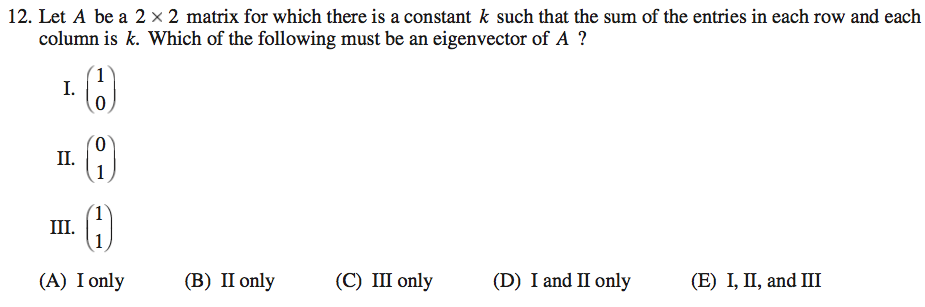
\includegraphics[scale=0.5]{0568_12}

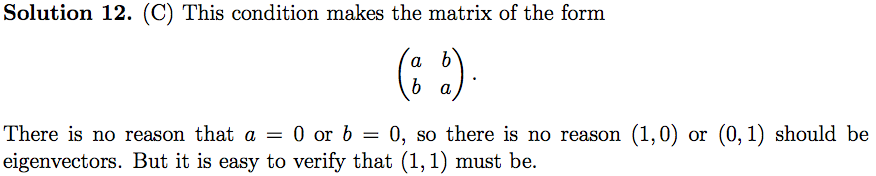
\includegraphics[scale=0.5]{0568_12s}

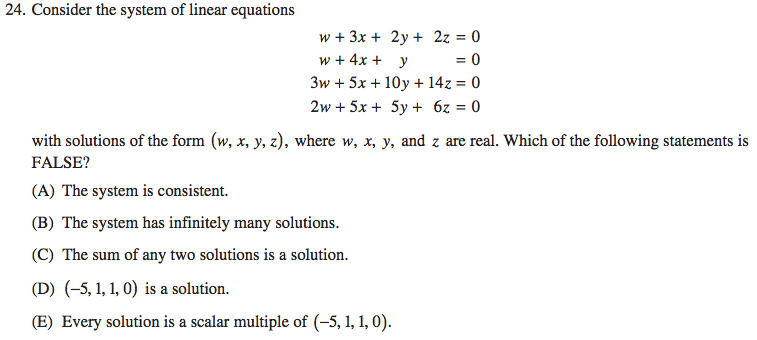
\includegraphics[scale=0.65]{1268_24}

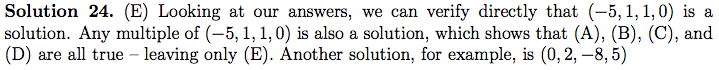
\includegraphics[scale=0.65]{1268_24s}

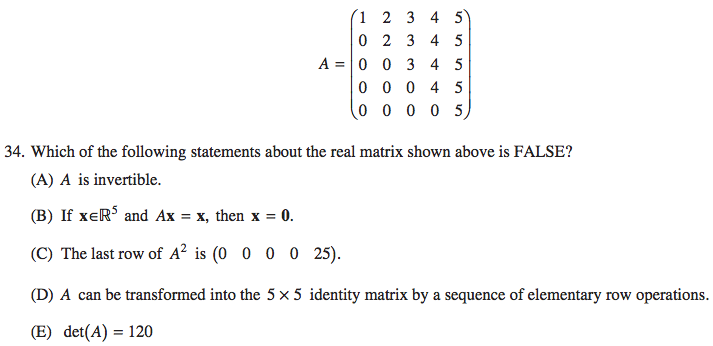
\includegraphics[scale=0.65]{1268_34}

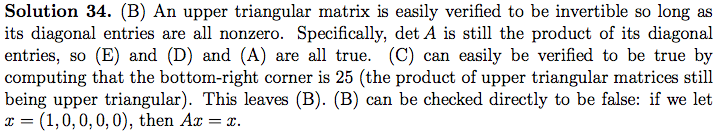
\includegraphics[scale=0.65]{1268_34s}

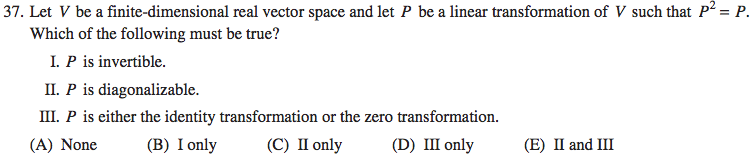
\includegraphics[scale=0.65]{1268_37}

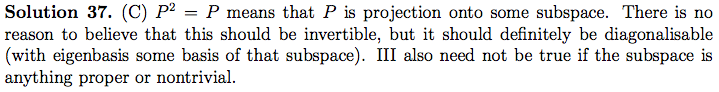
\includegraphics[scale=0.65]{1268_37s}

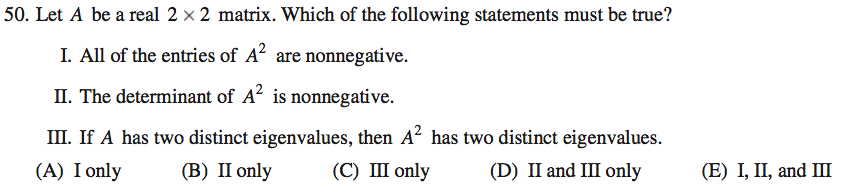
\includegraphics[scale=0.5]{0568_50}

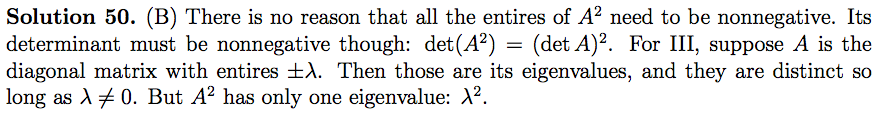
\includegraphics[scale=0.5]{0568_50s}

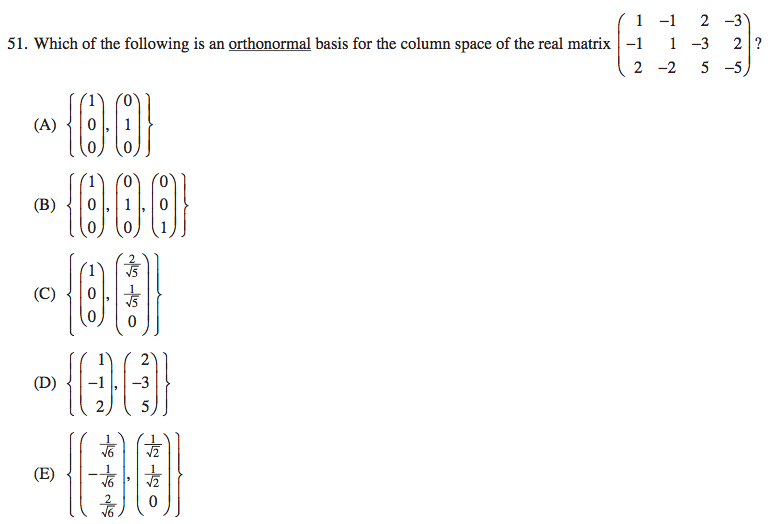
\includegraphics[scale=0.65]{1268_51}

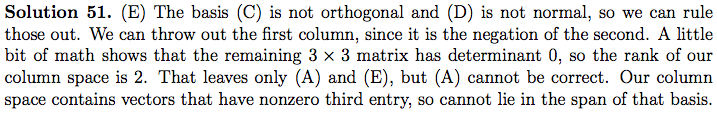
\includegraphics[scale=0.65]{1268_51s}

%%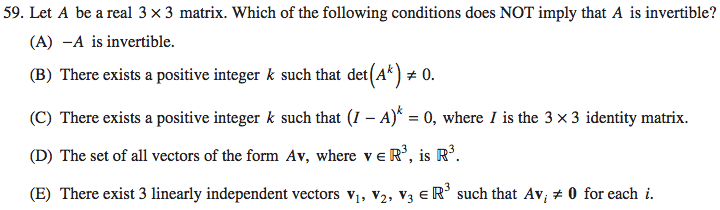
\includegraphics[scale=0.65]{1268_59}
%
%%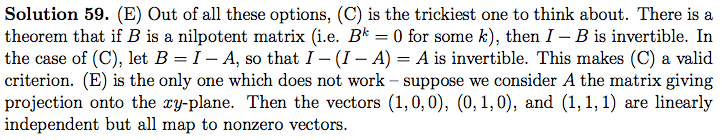
\includegraphics[scale=0.65]{1268_59s}

%
%
%
%
%

%\end{document}



